\section{Analiza Wymagań}
\subsection{Opis problemu.}
\begin{par}
	Tematem pracy jest zaprojektowanie i implementacja systemu podejmującego decyzje w prostej grze platformowej.
	Celem gry jest przejście dwuwymiarowej planszy z przeszkodami i przeciwnikami aż do jej końca, przy czym wynik końcowy może
	zostać oceniony również przez np. ilość zebranych punktów.
	Efektem pracy powinien być algorytm genetyczny który ten problem rozwiązuje i optymalizuje.
	\newline
	Ogólne wymogi dotyczące systemu:
	\begin{itemize}
		\item
			System składa się z w pełni grywalnego silnika gry, wzorowanego na rozwiązaniach w klasycznych grach platformowych.
			Oprócz podstawowego sterowania postacią za pomocą klawiszy, użytkownik powinien mieć możliwość uruchomienia gry w tryb sztucznej inteligencji,
			która wówczas sama podejmuje akcje w grze, wówczas zgodnie z parametrami ustawionymi w aplikacji, uruchamiana jest procedura treningu osobników.
		\item
			Do wyniku końcowego mogą być brane pod uwagę również inne zdarzenia takie jak ilość zebranych obiektów na planszy, bądź 
			pokonani przeciwnicy.
			Funkcja przystosowania zależeć będzie od rożnych czynników, a ustawienie odpowiednich wag może nakierować algorytm na określoną ścieżkę rozwoju.
			Oprócz tego elastyczna implementacja mutacji, krzyżowania oraz metody selekcji pozwoli na łatwą podmianę całej metody, dzięki czemu łatwo będzie można zweryfikować
			efektywność konkretnych podejść np. w krzyżowaniu bądź selekcji.
		\item
			Oprócz tego należy zdefiniować format danych przechowujący np. całą populację w celach archiwizacji, bądź tworzenia tzw. logów. 
			Dodatkowo, moduł pozwalający na łatwą wizualizację postępów posłuży jako dobra warstwa prezentacyjna postępu algorytmu w czasie.
	\end{itemize}
\end{par}

\begin{par}
	Sam pomysł stworzenia sztucznej inteligencji do gry platformowej w czasie rzeczywistym został już wcześniej wielokrotnie powołany do życia, m.in. jako projekt MarioAI,
	który w chwili obecnej funkcjonuje jako turniej dla programistów. Uczestnicy mogą implementować własne rozwiazania i porównywać wyniki z innymi uczestnikami.
	Samo zgłoszenie składa się z implementacji własnej klasy odpowiedzialnej za podejmowanie decyzji.
	Strona domowa projektu znajduje się pod adresem www.marioai.org.
\end{par}

\subsection{Wstępne założenia oraz diagram klas}
\begin{par}
	Aby dobrze zrealizować część odpowiedzialną za sterowanie postacią, należy użyć klasy pośredniej pomiędzy warstwą logiki silnika gry, a warstwą komunikacji z graczem. 
	Wówczas możemy łatwo zmienić źródło sygnałów wysyłanych do postaci z bezpośrednich zdarzeń z klawiatury na akcje przechowywane przez chromosom. 
	\subsubsection{Projekt Chromosomu}
	Kolejnym ważnym elementem jest odpowiednie zaprojektowanie chromosomu. 
	Dwa najbardziej trafne rozwiązania opierają się na dwóch zmiennych występujących w środowisku gry:
	\begin{enumerate}
	\item
	{\bf Czas który upłynął od rozpoczęcia danej instancji gry. }
	\begin{par}
	Wówczas akcje zostawałyby podejmowane w oparciu o aktualy czas w grze, a sama tablica akcji musiałaby przechowywać akcje których wykonanie następowałoby po kolei z pewnym interwałem, np. 30 ms. 
	Warto zauważyć że dzięki temu iż przebieg symulacji nie zależy od pozycji gracza, mamy swobodę ruchu, a jeśli to korzystne możemy założyć iż dobrym rozwiązanie w niektórych przypadkach będzie np. odczekanie określonego czasu, bądź powrót do miejsca w którym już byliśmy.
	Istotną wadą tego rozwiązania była duża podatność algorytmu na zapętlanie sie, lub wykonywanie dużej ilości mało przydatnych ruchów. 
	Jeśli chcielibyśmy dobrze zaprojektować taki algorytm musielibyśmy brać pod uwagę fakt, iż średnio przy równym prawdopodobieństwie ruchu w lewo jak i prawo, postać będzie przesuwała się bardzo powoli, bądź na dłuższą metę stała w miejscu.
	Wymagane wówczas byłoby takie zaprojektowanie algorytmu, gdzie ruch w kierunku końca planszy, oraz czas dościa do końca miałyby kluczowe znaczenie przy wyliczaniu funkcji przystosowania.
	Innym utrudnieniem może być krzyżowanie takich chromosomów. Ponieważ akcje postaci w większości przypadków mają sens w kontekście jej aktualnego położenia, o tyle klasyczne krzyżowanie ''cięcia'' chromosomu na dwie części jest nieefektywne.
	Otrzymamy wówczas niespójny ciąg ruchów, które będą miały niewiele wspólnego z aktualną pozycją gracza na mapie.
	Można temu zapobiec zapewniając łączenie się chromosomów jedynie w punktach w których postać w obu momentach znajduje się w tym samym lub zbliżonym miejscu.
	Komplikuje to jednak pozostałe mechanizmy selekcji i szukania punktu łączenia. 
	Przeszukiwanie punktów wspólnych można zrealizować w czasie $O(n*log_2n)$ najpierw sortując tablice obu osobników odpowiadające za ruch w chromosomie. 
	Tablice sortujemy względem współrzędnej X aktualnego położenia gracza dla każdej z akcji, a następnie liniowo przechodząc po obu tablicach osobników, szukając punktów wspólnych.
	Rozwiązanie to jest możliwe do zrealizowania, jednak bez skutecznej metody eliminacji powyższych problemów, może ona osiągać skuteczne wyniki wolniej.
	Wstępny schemat takiego rozwiązania mógłby wówczas wyglądać tak:
	\begin{figure}[h]
	\centering
	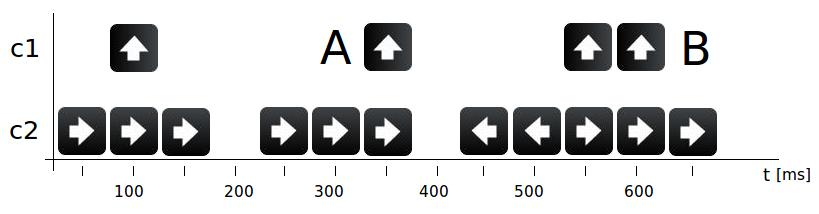
\includegraphics[width=\textwidth]{obrazki/sterowanie.jpg}
	\caption{Sterowanie względem czasu.}
	\label{fig:sterowanie}
	\end{figure}
	\end{par}
	\item
	{\bf Aktualna pozycja gracza.}
	\begin{par}
		O ile poprzednie rozwiązanie dawało większą swobodę ruchu po mapie, to było jednak mało optymalne pod względem osiągania szybko dobrych wyników.
		Jeśli założymy iż akcje przechowywane w chromosomie mają być aktywowane w momencie osiągnięcia przez gracza danej pozycji na osi X mapy, wówczas uprościmy cały mechanizm krzyżowania (już nie musimy szukać punktów wspólnych, gdyż dwa dowolne indeksy w obu tablicach $i,j$ gwarantują nam takie samo położenie gracza na mapie gdy $i=j$.
		Innym udogodnieniem będzie uproszczenie samego typu przechowywanych danych. Ponieważ rezygnujemy z postojów i ruchu w lewo, równie dobrze możemy zrezygnować z tablicy przechowującej te informacje.
		\begin{figure}[h]
		\centering
		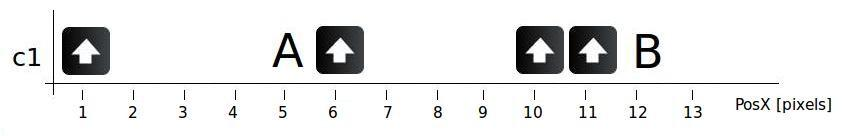
\includegraphics[width=\textwidth]{obrazki/sterowanie2.jpg}
		\caption{Sterowanie względem czasu.}
		\label{fig:sterowanie}
		\end{figure}
		Warto zauważyć iż gwarantuje nam to stały rozmiar tablicy, równy szerokości planszy w pikselach, co nawet dla średnich map, nie będzie dużym obciążeniem pamięciowym jeśli założymy iż akcje są przechowywane jako typy danych char(1 bajt). 
		Problem może stać się bardziej znaczący gdy zechcemy trenować algorytm na dużych mapach rzędu 10000 pixeli szerokości, do tego przechowując informacje o poprzednich populacjach w celach wizualizacji postępu.
		Wówczas populacja składająca się z 200 osobników, przy zapamietywaniu poprzednich populacji (500) może już zajmować znaczną część pamięci.
		Przy założeniu iż każda akcja przetrzymywana jest na dwóch bitach, otrzymujemy w zaokrągleniu:
		$10000*200*1000/4$ bajtów $= 476Mb$.
		Przechowywanie pojedynczej informacji jedynie na dwóch bitach jest możliwe z dwóch powodów:
		\begin{itemize}	
		\item
			Musimy przechowywać jedynie informację akcjach specjalnych czyli skoku i przyspieszenia.
		\item
			Możemy łatwo skonstruować klasę opakowującą tablicę, która za pomocą operacji na bitach może łatwo upakować informację o 4 pixelach do jednego bajtu.
		\end{itemize}

	\end{par}
	\end{enumerate}
	\begin{par}
		Wstępne założenia zakładają ruch postaci tylko w jedną stronę (prawo) oraz dwa klawisze akcji odpowiadające za skok oraz przyspieszenie, jednak warto zastanowić się nad ewentualną rozbudową chromosomu Sam chromosom składać się będzie z dwóch tablic danych, odpowiadających za akcje.

	\end{par}
	\begin{figure}[h]
	\centering
	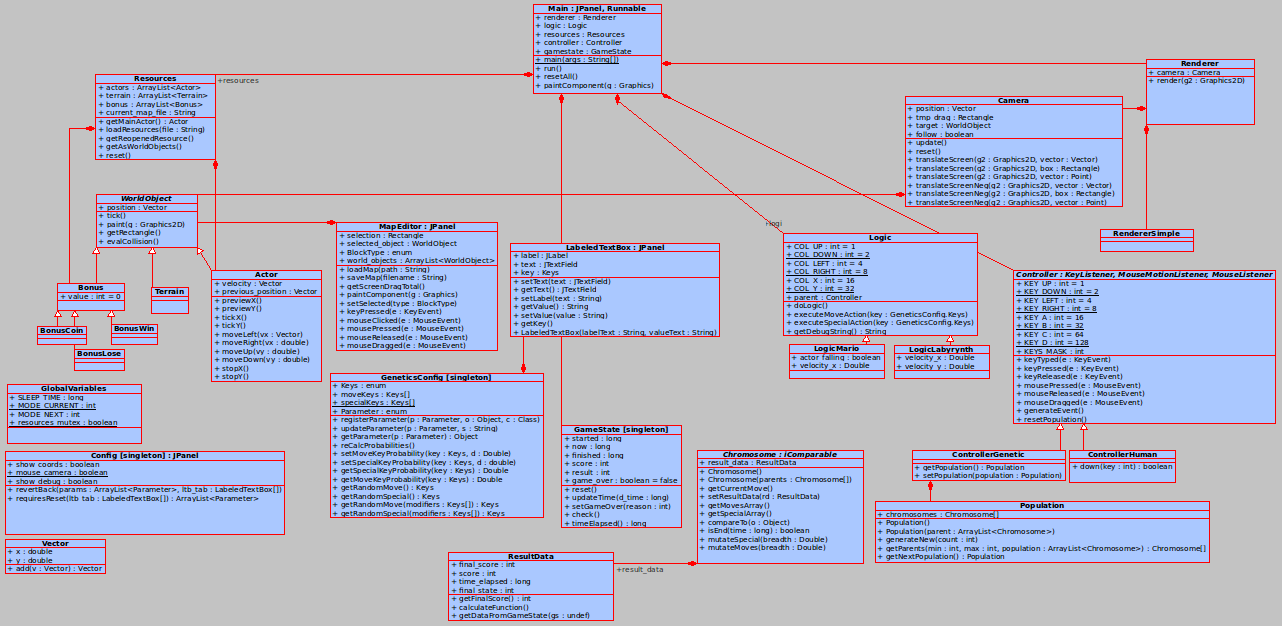
\includegraphics[width=\textwidth]{obrazki/diagram_klas.png}
	\caption{Diagram Klas.}
	\label{fig:diagram_klas}
	\end{figure}
\end{par}
